% Options for packages loaded elsewhere
\PassOptionsToPackage{unicode}{hyperref}
\PassOptionsToPackage{hyphens}{url}
%
\documentclass[
]{article}
\usepackage{amsmath,amssymb}
\usepackage{lmodern}
\usepackage{iftex}
\ifPDFTeX
  \usepackage[T1]{fontenc}
  \usepackage[utf8]{inputenc}
  \usepackage{textcomp} % provide euro and other symbols
\else % if luatex or xetex
  \usepackage{unicode-math}
  \defaultfontfeatures{Scale=MatchLowercase}
  \defaultfontfeatures[\rmfamily]{Ligatures=TeX,Scale=1}
\fi
% Use upquote if available, for straight quotes in verbatim environments
\IfFileExists{upquote.sty}{\usepackage{upquote}}{}
\IfFileExists{microtype.sty}{% use microtype if available
  \usepackage[]{microtype}
  \UseMicrotypeSet[protrusion]{basicmath} % disable protrusion for tt fonts
}{}
\makeatletter
\@ifundefined{KOMAClassName}{% if non-KOMA class
  \IfFileExists{parskip.sty}{%
    \usepackage{parskip}
  }{% else
    \setlength{\parindent}{0pt}
    \setlength{\parskip}{6pt plus 2pt minus 1pt}}
}{% if KOMA class
  \KOMAoptions{parskip=half}}
\makeatother
\usepackage{xcolor}
\IfFileExists{xurl.sty}{\usepackage{xurl}}{} % add URL line breaks if available
\IfFileExists{bookmark.sty}{\usepackage{bookmark}}{\usepackage{hyperref}}
\hypersetup{
  pdftitle={Hypergeometric Distribution},
  hidelinks,
  pdfcreator={LaTeX via pandoc}}
\urlstyle{same} % disable monospaced font for URLs
\usepackage[margin=1in]{geometry}
\usepackage{color}
\usepackage{fancyvrb}
\newcommand{\VerbBar}{|}
\newcommand{\VERB}{\Verb[commandchars=\\\{\}]}
\DefineVerbatimEnvironment{Highlighting}{Verbatim}{commandchars=\\\{\}}
% Add ',fontsize=\small' for more characters per line
\usepackage{framed}
\definecolor{shadecolor}{RGB}{248,248,248}
\newenvironment{Shaded}{\begin{snugshade}}{\end{snugshade}}
\newcommand{\AlertTok}[1]{\textcolor[rgb]{0.94,0.16,0.16}{#1}}
\newcommand{\AnnotationTok}[1]{\textcolor[rgb]{0.56,0.35,0.01}{\textbf{\textit{#1}}}}
\newcommand{\AttributeTok}[1]{\textcolor[rgb]{0.77,0.63,0.00}{#1}}
\newcommand{\BaseNTok}[1]{\textcolor[rgb]{0.00,0.00,0.81}{#1}}
\newcommand{\BuiltInTok}[1]{#1}
\newcommand{\CharTok}[1]{\textcolor[rgb]{0.31,0.60,0.02}{#1}}
\newcommand{\CommentTok}[1]{\textcolor[rgb]{0.56,0.35,0.01}{\textit{#1}}}
\newcommand{\CommentVarTok}[1]{\textcolor[rgb]{0.56,0.35,0.01}{\textbf{\textit{#1}}}}
\newcommand{\ConstantTok}[1]{\textcolor[rgb]{0.00,0.00,0.00}{#1}}
\newcommand{\ControlFlowTok}[1]{\textcolor[rgb]{0.13,0.29,0.53}{\textbf{#1}}}
\newcommand{\DataTypeTok}[1]{\textcolor[rgb]{0.13,0.29,0.53}{#1}}
\newcommand{\DecValTok}[1]{\textcolor[rgb]{0.00,0.00,0.81}{#1}}
\newcommand{\DocumentationTok}[1]{\textcolor[rgb]{0.56,0.35,0.01}{\textbf{\textit{#1}}}}
\newcommand{\ErrorTok}[1]{\textcolor[rgb]{0.64,0.00,0.00}{\textbf{#1}}}
\newcommand{\ExtensionTok}[1]{#1}
\newcommand{\FloatTok}[1]{\textcolor[rgb]{0.00,0.00,0.81}{#1}}
\newcommand{\FunctionTok}[1]{\textcolor[rgb]{0.00,0.00,0.00}{#1}}
\newcommand{\ImportTok}[1]{#1}
\newcommand{\InformationTok}[1]{\textcolor[rgb]{0.56,0.35,0.01}{\textbf{\textit{#1}}}}
\newcommand{\KeywordTok}[1]{\textcolor[rgb]{0.13,0.29,0.53}{\textbf{#1}}}
\newcommand{\NormalTok}[1]{#1}
\newcommand{\OperatorTok}[1]{\textcolor[rgb]{0.81,0.36,0.00}{\textbf{#1}}}
\newcommand{\OtherTok}[1]{\textcolor[rgb]{0.56,0.35,0.01}{#1}}
\newcommand{\PreprocessorTok}[1]{\textcolor[rgb]{0.56,0.35,0.01}{\textit{#1}}}
\newcommand{\RegionMarkerTok}[1]{#1}
\newcommand{\SpecialCharTok}[1]{\textcolor[rgb]{0.00,0.00,0.00}{#1}}
\newcommand{\SpecialStringTok}[1]{\textcolor[rgb]{0.31,0.60,0.02}{#1}}
\newcommand{\StringTok}[1]{\textcolor[rgb]{0.31,0.60,0.02}{#1}}
\newcommand{\VariableTok}[1]{\textcolor[rgb]{0.00,0.00,0.00}{#1}}
\newcommand{\VerbatimStringTok}[1]{\textcolor[rgb]{0.31,0.60,0.02}{#1}}
\newcommand{\WarningTok}[1]{\textcolor[rgb]{0.56,0.35,0.01}{\textbf{\textit{#1}}}}
\usepackage{graphicx}
\makeatletter
\def\maxwidth{\ifdim\Gin@nat@width>\linewidth\linewidth\else\Gin@nat@width\fi}
\def\maxheight{\ifdim\Gin@nat@height>\textheight\textheight\else\Gin@nat@height\fi}
\makeatother
% Scale images if necessary, so that they will not overflow the page
% margins by default, and it is still possible to overwrite the defaults
% using explicit options in \includegraphics[width, height, ...]{}
\setkeys{Gin}{width=\maxwidth,height=\maxheight,keepaspectratio}
% Set default figure placement to htbp
\makeatletter
\def\fps@figure{htbp}
\makeatother
\setlength{\emergencystretch}{3em} % prevent overfull lines
\providecommand{\tightlist}{%
  \setlength{\itemsep}{0pt}\setlength{\parskip}{0pt}}
\setcounter{secnumdepth}{-\maxdimen} % remove section numbering
\ifLuaTeX
  \usepackage{selnolig}  % disable illegal ligatures
\fi

\title{Hypergeometric Distribution}
\usepackage{etoolbox}
\makeatletter
\providecommand{\subtitle}[1]{% add subtitle to \maketitle
  \apptocmd{\@title}{\par {\large #1 \par}}{}{}
}
\makeatother
\subtitle{XDASI Fall 2021}
\author{}
\date{\vspace{-2.5em}10/14/2021}

\begin{document}
\maketitle

{
\setcounter{tocdepth}{2}
\tableofcontents
}
\hypertarget{hypergeometric-distribution}{%
\section{Hypergeometric
distribution}\label{hypergeometric-distribution}}

The hypergeometric distribution is similar to the \emph{binomial
distribution}, except it defines the \emph{probability of obtaining
\(x\) independent successes} when sampling \emph{\textbf{without
replacement}}. It is classically described in terms of an urn containing
some black balls and some white balls. The hypergeometric distribution
will tell us how likely it is that a handful of balls picked from the
urn contains a certain number of black (or white) balls.

\hypertarget{example-go-term-enrichment}{%
\subsection{Example: GO-term
enrichment}\label{example-go-term-enrichment}}

In our field, probably the most common application of the hypergeometric
distribution is to test whether a set of genes of interest (e.g.~up- or
down-regulated genes in a differential gene expression analysis) is
enriched for a specific functional annotation (e.g.~GO term).

To test this, we need to ask whether the observed overlap is different
from what we would expect if we picked the same number of genes at
random from the genome. What would this be? We can use set theory to
figure this out. Let's visualize the problem:

\begin{figure}
\centering
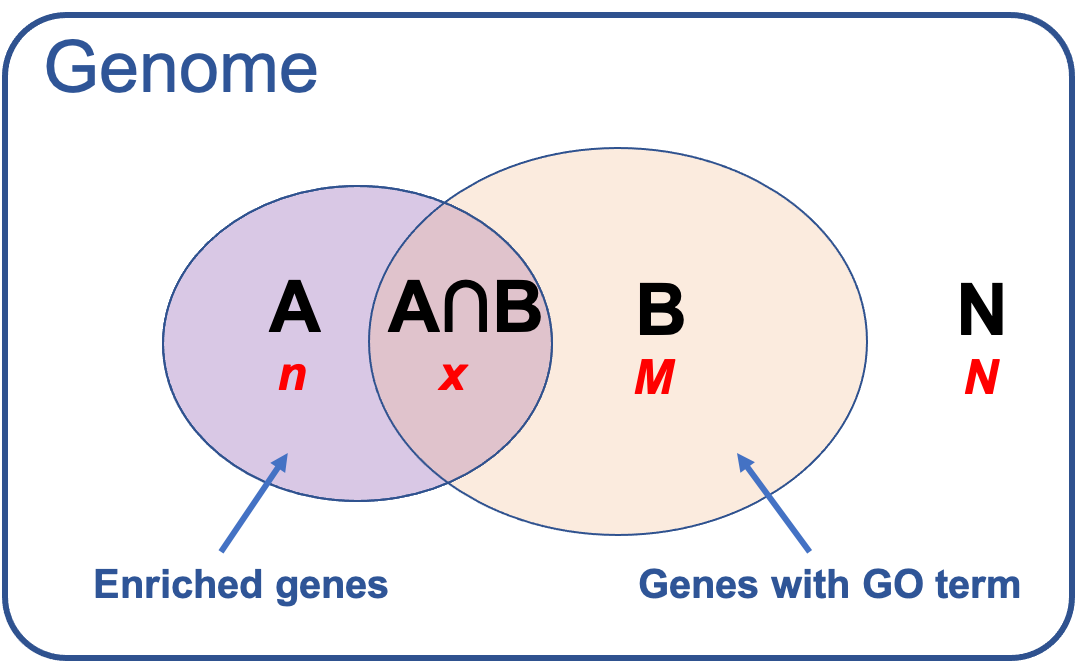
\includegraphics[width=0.4\textwidth,height=\textheight]{hypergeometric.png}
\caption{\textbf{Overlap between two sets of genes in the genome}}
\end{figure}

Our question is whether the overlap between the two sets of genes is
greater than (or less than) expected by chance. Under independence, we
know that:

\[Pr[A \cap B] = Pr[A]*Pr[B]\]

We can use a hypergeometric test to answer this question. The question
is formulated in this way:

\textbf{\emph{If we pick \(n\) out of \(N\) total items (Set A), what is
the chance that \(x\) of them would also be contained in \(M\) (Set B),
if the two sets were independent?}}

To answer this, we need to know just a few things:

\begin{itemize}
\tightlist
\item
  \(N\): the total number of selectable items in the genome
\item
  \(n\): the number of items in Set \(A\)
\item
  \(M\): the number of items in Set \(B\)
\item
  \(x\): the overlap between Set A and Set B (\(A \cap B\))
\end{itemize}

\hypertarget{hypergeometric-pdf}{%
\subsection{Hypergeometric PDF}\label{hypergeometric-pdf}}

Sampling without replacement means that we are picking a particular set
of items from a finite set of total items. Therefore, each trial affects
the probability of the next outcome -- in other words, we need an
equation to find the relative frequency of \(x\) in a shrinking sample
space. (If the population were infinite, then this would essentially be
the same as sampling with replacement, since the sample would not make a
dent in the remaining number of individuals to choose from.)

The PDF is defined as:

\[ f(x) = P(X = x) = {M \choose x}{N - M \choose n - x}\bigg/{N \choose n} \]

where:

\begin{itemize}
\tightlist
\item
  \(x \in \{0,1,2,...,n\}\) is the number of ``successful'' trials
\item
  \(N \in \{1,2,...,N\}\) is the total number of selectable items
\item
  \(M \in \{0,1,2,...,N\}\) is the total number of possible
  ``successful'' outcomes (the number of items in the group we are
  comparing against)
\item
  \(n \in \{0,1,2,...,N\}\) is the number of items sampled
\end{itemize}

The random variable \(x\) represents the overlap between the two sets
(\(A \cap B\)), \(n\) is Set \(A\), and \(M\) is Set \(B\). Here, Set
\(B\) is defined as ``success'' and Set \(A\) is the sample we are
asking about.

The \textbf{lower-tail} probability is the probability that
\textbf{\emph{fewer}} than \(x\) overlaps are observed (depletion), and
the \textbf{upper-tail} probability is the probability that
\textbf{\emph{more}} than \(x\) overlaps are observed (enrichment).

The components of the equation are:

\begin{itemize}
\tightlist
\item
  \(\binom{M}{x}\): the number of ways to get (\(A \cap B\)) out of
  \(B\) items
\item
  \(\binom{N - M}{n - x}\): the number of ways to get
  (\(A\ \ NOT\ \ B\)) out of (\(N\ \ NOT\ \ B\)) items
\item
  \(\binom{N}{n}\): the number of ways to get \(A\) out of \(N\) items
\end{itemize}

\begin{figure}
\centering
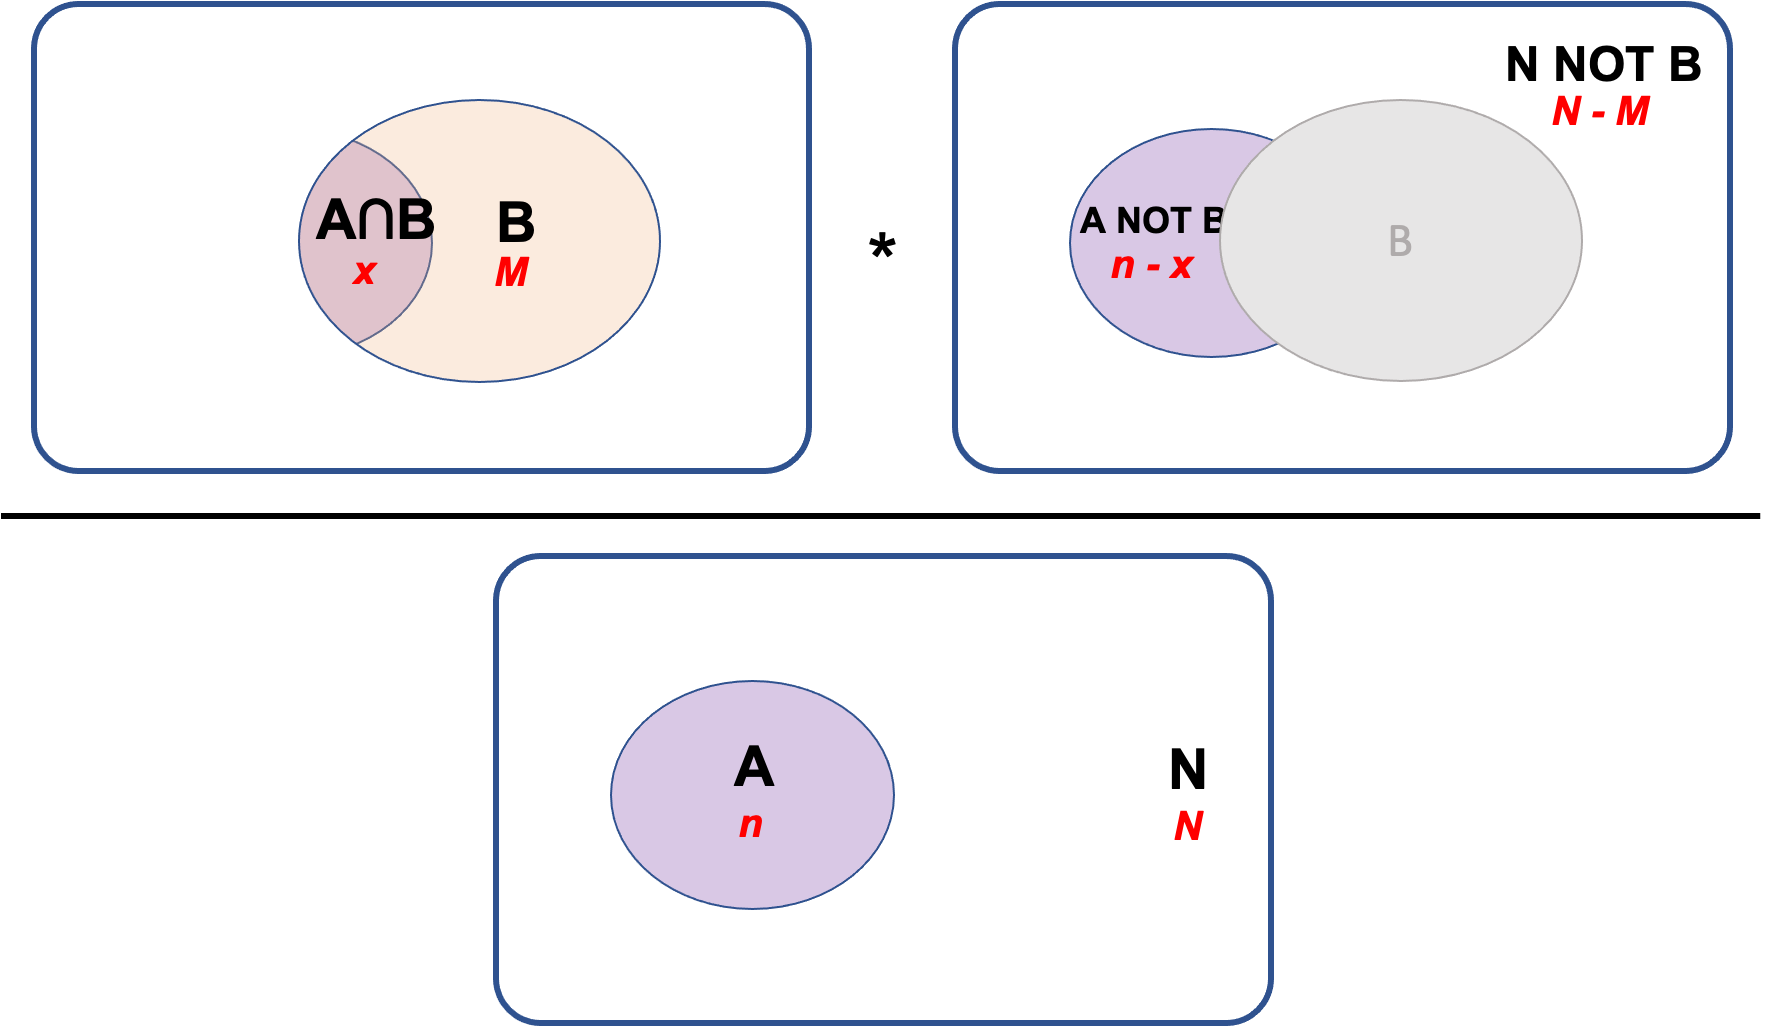
\includegraphics[width=0.5\textwidth,height=\textheight]{hyper_choose.png}
\caption{\textbf{Hypergeometric formula}}
\end{figure}

\hypertarget{hypergeometric-test}{%
\subsection{Hypergeometric test}\label{hypergeometric-test}}

The \texttt{hyper} family of functions in R does not observe the usual
naming convention, which is a bit confusing at first, but the variables
are the same.

For example{[}\^{}1{]}, let's say we have a list of 59 genes that are
predicted to be regulated by the mouse E2F transcription factor, and we
want to know whether they are enriched for genes involved in the cell
cycle. There are 13,588 genes with some GO annotation in the mouse
genome, and 611 of them are annotated with the term ``cell cycle''. We
find that 19 out of our 59 genes are annotated with the GO term ``cell
cycle''.

Is the list of predicted E2F targets significantly enriched for the GO
term ``cell cycle''? We can figure this out in the following way:

\begin{Shaded}
\begin{Highlighting}[]
\FunctionTok{help}\NormalTok{(phyper)}

\CommentTok{\# hypergeometric CDF in R is defined as: }
\CommentTok{\#   p(x) = choose(m, x) choose(n, k{-}x) / choose(m+n, k)}

\CommentTok{\# the formula is:}
\CommentTok{\#   phyper(q, m, n, k, lower.tail = T/F)}

\CommentTok{\# Instead, we will use: }
\CommentTok{\#   phyper(Overlap{-}1, SetB, N {-} SetB, SetA, lower.tail= FALSE)}
\NormalTok{Overlap }\OtherTok{=} \DecValTok{19}  \CommentTok{\# predicted genes with GO term}
\NormalTok{A }\OtherTok{=} \DecValTok{59}     \CommentTok{\# predicted E2F targets}
\NormalTok{B }\OtherTok{=} \DecValTok{611}    \CommentTok{\# genes with GO term}
\NormalTok{N }\OtherTok{=} \DecValTok{13588}     \CommentTok{\# total annotated genes}

\CommentTok{\# Expected overlap based on the null hypothesis:}
\CommentTok{\# [\# genes in (A AND B)] = [\# genes in A] * [\# genes in B] / N}
\NormalTok{exp.overlap }\OtherTok{=}\NormalTok{ A }\SpecialCharTok{*}\NormalTok{ B }\SpecialCharTok{/}\NormalTok{ N}
\FunctionTok{print}\NormalTok{(}\FunctionTok{paste}\NormalTok{(}\StringTok{"Expected overlap ="}\NormalTok{, }\FunctionTok{round}\NormalTok{(exp.overlap,}\DecValTok{2}\NormalTok{)))}
\end{Highlighting}
\end{Shaded}

\begin{verbatim}
## [1] "Expected overlap = 2.65"
\end{verbatim}

\begin{Shaded}
\begin{Highlighting}[]
\CommentTok{\# Fold{-}enrichment:}
\NormalTok{fold.enrichment }\OtherTok{=}\NormalTok{ ( Overlap}\SpecialCharTok{/}\NormalTok{A ) }\SpecialCharTok{/}\NormalTok{ ( B}\SpecialCharTok{/}\NormalTok{N )}
\FunctionTok{print}\NormalTok{(}\FunctionTok{paste}\NormalTok{(}\StringTok{"Fold{-}enrichment ="}\NormalTok{, }\FunctionTok{round}\NormalTok{(fold.enrichment,}\DecValTok{2}\NormalTok{)))}
\end{Highlighting}
\end{Shaded}

\begin{verbatim}
## [1] "Fold-enrichment = 7.16"
\end{verbatim}

\begin{Shaded}
\begin{Highlighting}[]
\CommentTok{\# P(enrichment) = upper{-}tail probability: P(X \textgreater{}= x)}
\CommentTok{\# Note: We use Overlap{-}1, otherwise we are asking for P(X \textgreater{} x)}
\CommentTok{\#       since this is a discrete distribution}
\FunctionTok{phyper}\NormalTok{(Overlap}\DecValTok{{-}1}\NormalTok{, B, N }\SpecialCharTok{{-}}\NormalTok{ B, A, }\AttributeTok{lower.tail=} \ConstantTok{FALSE}\NormalTok{)}
\end{Highlighting}
\end{Shaded}

\begin{verbatim}
## [1] 4.989683e-12
\end{verbatim}

\begin{Shaded}
\begin{Highlighting}[]
\CommentTok{\# same using PDF instead}
\FunctionTok{sum}\NormalTok{(}\FunctionTok{dhyper}\NormalTok{( Overlap}\SpecialCharTok{:}\NormalTok{A, B, N }\SpecialCharTok{{-}}\NormalTok{ B, A ))}
\end{Highlighting}
\end{Shaded}

\begin{verbatim}
## [1] 4.989683e-12
\end{verbatim}

\hypertarget{fishers-exact-test}{%
\subsection{Fisher's Exact Test}\label{fishers-exact-test}}

The hypergeometric test is the same as a one-tailed Fisher's exact test:

\begin{Shaded}
\begin{Highlighting}[]
\CommentTok{\# set up the contingency table with the overlap in the top left corner}
\CommentTok{\# first row is the predicted targets}
\NormalTok{A.not.B }\OtherTok{=}\NormalTok{ A}\SpecialCharTok{{-}}\NormalTok{Overlap}
\NormalTok{B.not.A }\OtherTok{=}\NormalTok{ B}\SpecialCharTok{{-}}\NormalTok{Overlap}
\NormalTok{N.not.AB }\OtherTok{=}\NormalTok{ N }\SpecialCharTok{{-}}\NormalTok{ B }\SpecialCharTok{{-}}\NormalTok{ A.not.B}
\NormalTok{contingency.table }\OtherTok{=} \FunctionTok{rbind}\NormalTok{(}\FunctionTok{c}\NormalTok{(Overlap, A.not.B),}
                          \FunctionTok{c}\NormalTok{(B.not.A, N.not.AB))}
\FunctionTok{rownames}\NormalTok{(contingency.table) }\OtherTok{=} \FunctionTok{c}\NormalTok{(}\StringTok{"target"}\NormalTok{,}\StringTok{"not.target"}\NormalTok{)}
\FunctionTok{colnames}\NormalTok{(contingency.table) }\OtherTok{=} \FunctionTok{c}\NormalTok{(}\StringTok{"GO"}\NormalTok{,}\StringTok{"not.GO"}\NormalTok{)}
\NormalTok{contingency.table}
\end{Highlighting}
\end{Shaded}

\begin{verbatim}
##             GO not.GO
## target      19     40
## not.target 592  12937
\end{verbatim}

\begin{Shaded}
\begin{Highlighting}[]
\CommentTok{\# Is the overlap greater than expected by chance?}
\FunctionTok{fisher.test}\NormalTok{(contingency.table, }\AttributeTok{alternative=}\StringTok{"greater"}\NormalTok{)}
\end{Highlighting}
\end{Shaded}

\begin{verbatim}
## 
##  Fisher's Exact Test for Count Data
## 
## data:  contingency.table
## p-value = 4.99e-12
## alternative hypothesis: true odds ratio is greater than 1
## 95 percent confidence interval:
##  6.204117      Inf
## sample estimates:
## odds ratio 
##   10.37524
\end{verbatim}

\end{document}
